% === Cours de Java
% === Chapitre : Survol 

\subsection{Code modulaire (premier survol)}

\begin{frame}[fragile]{Les variables}
Les types disponibles
\begin{center}
\begin{tabular}{r|l}
En Algorithmique & En  Java \\ \hline
Entier & \java|int| \\ 
R�el & \java|double| \\ 
Chaine & \java|char|, \java|String| \\ 
Bool�en & \java|boolean| \\  
\end{tabular} 
\end{center}
\end{frame}

\begin{frame}[fragile]{Les calculs}
Op�rateurs :
\begin{center}
	\Large
    \java|+| \java|-| \java|*| \java|/| \java|%|  
\end{center}
\end{frame}

\begin{frame}[fragile]{Variable}
	On peut stocker une valeur, le r�sultat d'un calcul dans une \emph{variable}
	
	\bigskip
	
	\emph{D�claration}\\
\begin{Java}
   typeVariable nomVariable;
\end{Java}

	\begin{itemize}
	\item Exemples :
\begin{Java}
   int nb1;
   String nom;
\end{Java}
	\end{itemize}
\end{frame}


\begin{frame}[fragile]{Variable}
	\emph{Assignation}\\
	Via le symbole \java|=|
	\begin{itemize}
	\item Exemples :
\begin{Java}
   nb1 = 1;
   nb1 = 3+4;
   nom = "Java";
   moyenne = (nombre1 + nombre2) / 2.0;
   d� = Math.random() * 6 + 1
\end{Java}
	\end{itemize}
\end{frame}


\imgfullh{../img/cut_and_fold_by_alltelleringet-d5jmcpu.jpg}
	{
		\begin{flushright}
			\vspace{3.5cm}
			\Large\bf\color{honeydew} D�couper le code
			\vspace{-3.5cm}
		\end{flushright}
		}
	{http://alltelleringet.deviantart.com/art/Cut-and-Fold-335286498}

\note{
	Expliquer pourquoi d�couper le code. Algo a une volont� d'expliquer que ce 
    d�coupage soit \textbf{naturel}. �vitons donc d'�crire des r�gles. 

    L'id�e c'est: r�utilisabilit�, scinder la difficult�, d�verminer, lisibilit�,
    r�partition du travail.

    On aime qu'une m�thode porte un nom explicite, r�solve un probl�me pr�cis et 
    clairement d�fini, qu'elle soit document�e, etc.
	}


\full[bluepigment]{
	\begin{center}
		\Large\color{white}\textbf{Appel} de m�thode
	\end{center}
}

\begin{frame}{Appel d'une m�thode}
Une m�thode est une \emph{boite noire}
\begin{center}
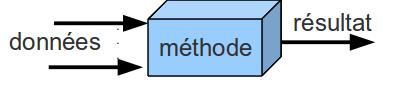
\includegraphics[scale=.6]{../img/methode}
\end{center}
Pour l'utiliser, il faut connaitre\,:
\begin{itemize}
\item son nom;
\item ce dont elle a besoin;
\item ce qu'elle retourne;
\item mais \emph{pas comment} elle fait;
\end{itemize}
\end{frame}

\imgfullh{../img/darkvador-magician.jpg}
{
		\begin{center}
			\color{white}\large
			Pas de \textbf{comment} ? \\
			Un simple \textbf{quoi}
		\end{center}
}
{https://www.flickr.com/photos/st3f4n/14480265204/sizes/l}

\begin{frame}[fragile]{Appel d'une m�thode}
� partir du code d'une \emph{autre classe} 
  \begin{itemize}
  \item \java|NomClasse.nomM�thode(...)|
  \item \emph{Exemples} :
    \begin{Java}
double racine = Math.sqrt(4.0);
double al�atoire = Math.random();
int nb = -10;
int absolu = Math.abs(nb);
    \end{Java}
  \end{itemize}
  \bigskip
  \textit{Un appel de m�thode au sein de la classe ne n�cessite pas de r�p�ter
  le nom de la classe}
\end{frame}

\full[bluepigment]{
	\begin{center}
		\Large\color{azuremist}\textbf{D�finition} d'une m�thode
	\end{center}
}

\begin{frame}[fragile]{D�finition d'une m�thode}
	\textbf{Syntaxe}
	\bigskip
\begin{Java}
	public static <typeRetour> nomM�thode ([param�tre, param�tre, ...]) {  
    // instructions
    <return r�sultat>;  
}
\end{Java}
\end{frame}




